\section{
    Сумма и пересечение линейных подпространств. Доказать, что указанные множества являются линейными подпространствами. Нахождение базисов для суммы и пересечения подпространств. Теорема о размерностях подпространств, суммы и пересечения.
}

\subsection{
    Сумма и пересечение линейных подпространств.
}   

\begin{definition}
    Пусть $\mathcal{H}_1$ и $\mathcal{H}_2$ - линейные подпространства в линейном пространстве $\mathcal{L}$. Множество $\mathcal{H}_1 + \mathcal{H}_2$ всех векторов $\vec{x}$ вида $\vec{x} = \vec{x_1} + \vec{x_2}$, где $\vec{x_1} \in \mathcal{H}_1$, $\vec{x_2} \in \mathcal{H}_2$, называют \textbf{\textit{суммой линейных подпространств}} $\mathcal{H}_1$ и $\mathcal{H}_2$. 
\end{definition}

\begin{figure}[H]
    \centering
    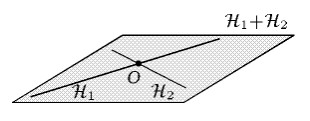
\includegraphics[scale=0.7]{images/4_1.jpg}
    \label{fig:picture_4_1}
    \caption{Сумма линейных подпространств.}
\end{figure}

\begin{definition}
    Пусть $\mathcal{H}_1$ и $\mathcal{H}_2$ - линейные подпространства в линейном пространстве $\mathcal{L}$. Множество $\mathcal{H}_1 \cap \mathcal{H}_2$ всех векторов $\vec{x}$, где $\vec{x} \in \mathcal{H}_1$ и $\vec{x} \in \mathcal{H}_2$, называют \textbf{\textit{пересечением линейных подпространств}} $\mathcal{H}_1$ и $\mathcal{H}_2$.
\end{definition}

\begin{figure}[H]
    \centering
    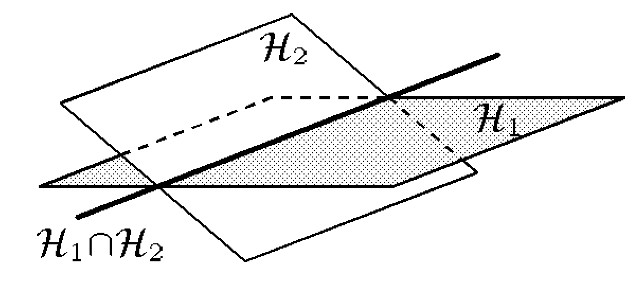
\includegraphics[scale=0.4]{images/4_2.jpg}
    \label{fig:picture_4_2}
    \caption{Пересечение линейных подпространств.}
\end{figure}


\newpage


\subsection{
    Доказать, что указанные множества (сумма и пересечение ЛПП) являются линейными подпространствами.
}

\begin{theorem}
    Сумма линейных подпространств данного линейного пространства является линейным подпространством в том же линейном пространстве.
\end{theorem}

\begin{proof}~

    Проверим, выполняются ли условия определения линейного подпространства:
    \begin{enumerate}[nosep]
        \item Рассмотрим два вектора $\vec{v}$ и $\vec{w}$ из множества $\mathcal{H}_1 + \mathcal{H}_2$. Согласно определению суммы линейных подпространств, имеют место представления $\vec{v} = \vec{x_1} + \vec{x_2}$, $\vec{w} = \vec{y_1} + \vec{y_2}$, где векторы $\vec{x_i}$, $\vec{y_i}$ принадлежат $\mathcal{H}_i$, $i = 1, 2$. Складывая эти равенства, получаем
        $$\vec{v} + \vec{w} = (\vec{x_1} + \vec{y_1}) + (\vec{x_2} + \vec{y_2}).$$
        Сумма $\vec{x_1} + \vec{y_1}$ векторов $\vec{x_1}$ и $\vec{y_1}$ линейного подпространства $\mathcal{H}_1$ принадлежит $\mathcal{H}_1$. Точно так же сумма $\vec{x_2} + \vec{y_2}$ векторов $\vec{x_2}$ и $\vec{y_2}$ линейного подпространства $\mathcal{H}_2$ принадлежит $\mathcal{H}_2$. Поэтому вектор $\vec{v} + \vec{w}$ принадлежит множеству $\mathcal{H}_1 + \mathcal{H}_2$.
        \item Произвольный вектор $\vec{v} \in \mathcal{H}_1 + \mathcal{H}_2$ имеет представление $\vec{v} = \vec{x_1} + \vec{x_2}$, где $\vec{x_1} \in \mathcal{H}_1$, $\vec{x_2} \in \mathcal{H}_2$. Для любого действительного числа $\lambda$ получаем равенства 
        $$\lambda \vec{v} = \lambda (\vec{x_1} + \vec{x_2}) = \lambda \vec{x_1} + \lambda \vec{x_2}.$$
        Так как вектор $\lambda \vec{x_1}$ принадлежит $\mathcal{H}_1$, а вектор $\lambda \vec{x_2}$ - $\mathcal{H}_2$, то вектор $\lambda \vec{u}$ является элементом множества $\mathcal{H}_1 + \mathcal{H}_2$.
    \end{enumerate}
    Мы доказали, что множество $\mathcal{H}_1 + \mathcal{H}_2$ замкнуто относительно линейных операций объемлющего линейного пространства и поэтому, согласно определению линейного подпространства, оно является линейным подпространством.
\end{proof}

\begin{theorem}
    Пересечение $\mathcal{H}_1 \cap \mathcal{H}_2$ двух линейных подпространств $\mathcal{H}_1$ и $\mathcal{H}_2$ в линейном пространстве $\mathcal{L}$ является линейным подпространством в $\mathcal{L}$.
\end{theorem}

\begin{proof}~

    Проверим, выполняются ли условия определения линейного подпространства:
    \begin{enumerate}[nosep]
        \item Если векторы $\vec{x_1}$ и $\vec{x_2}$ принадлежат $\mathcal{H}_1 \cap \mathcal{H}_2$, то каждый из этих векторов принадлежит как $\mathcal{H}_1$, так и $\mathcal{H}_2$. Поскольку $\mathcal{H}_1$ - линейное подпространство, то согласно определению линейного подпространства, заключаем, что вектор $\vec{x_1} + \vec{x_2}$, равный сумме векторов этого линейного подпространства, тоже принадлежит $\mathcal{H}_1$. Аналогично $\vec{x_1} + \vec{x_2} \in \mathcal{H}_2$, так как каждое из слагаемых является элементом линейного подпространства $\mathcal{H}_2$. Следовательно, $\vec{x_1} + \vec{x_2} \in \mathcal{H}_1 \cap \mathcal{H}_2$.
        \item Выберем произвольный вектор $\vec{x} \in \mathcal{H}_1 \cap \mathcal{H}_2$. Тогда $\vec{x} \in \mathcal{H}_1$ и $\vec{x} \in \mathcal{H}_2$. Так как $\mathcal{H}_1$ является линейным подпространством, то произведение элемента $\vec{x}$ этого линейного подпространства на произвольное действительное число $\lambda$ принадлежит $\mathcal{H}_1$. Но совершенно аналогично вектор $\lambda \vec{x}$ принадлежит и $\mathcal{H}_2$. Поэтому $\lambda \vec{x} \in \mathcal{H}_1 \cap \mathcal{H}_2$. 
    \end{enumerate}
    Итак, оба условия определения линейного подпространства выполнены. Следовательно, $\mathcal{H}_1 \cap \mathcal{H}_2$ является линейным подпространством.
\end{proof}


\newpage


\subsection{
    Нахождение базисов для суммы и пересечения подпространств.
}

\begin{theorem}
    Если $\{e\}$ - базис $\mathcal{L}_1$, $\{f\}$ - базис $\mathcal{L}_2$, $\ldots$, $\{g\}$ - базис $\mathcal{L}_k$, то $\sum_{j=1}^{k} L_j = span(e, f, \ldots, g)$.
\end{theorem}

\begin{proof}
    $\vec{x} = \underbrace{\vec{x_1}}_{\text{расклад. по $e$}} + \underbrace{\vec{x_2}}_{\text{расклад. по $f$}} + \ldots + \underbrace{\vec{x_k}}_{\text{расклад. по $g$}}$
\end{proof}

\begin{comment}
    Набор $(e, f, \ldots, g)$ может быть избыточен; нужны только ЛНЗ векторы.
\end{comment}

\begin{proposition}
    $\dim \sum_{j=1}^{k} \mathcal{L}_j = rank(e, f, \ldots, g)$.
\end{proposition}

Пусть $\mathcal{L}_1, \mathcal{L}_2, \ldots, \mathcal{L}_k$ заданы с помощью СЛАУ. Базисом суммы подпространств $\mathcal{L}_1 + \mathcal{L}_2 + \ldots + \mathcal{L}_k$ будет любая её ФСР. Базисом пересечения подпространств $\mathcal{L}_1 \cap \mathcal{L}_2 \cap \ldots \cap \mathcal{L}_k$ будет любая его ФСР.


\newpage


\subsection{
    Теорема о размерностях подпространств, суммы и пересечения.
}

\begin{theorem}
    Если $\mathcal{H}$ - линейное подпространство линейного пространства $\mathcal{L}$, то $\dim \mathcal{H} \leq \dim \mathcal{L}$. Если к тому же $\mathcal{H} \ne \mathcal{L}$, то $\dim \mathcal{H} < \dim \mathcal{L}$.
\end{theorem}

\begin{proof}~

    Любой базис линейного подпространства $\mathcal{H}$ является ЛНЗ системой векторов в линейном пространстве $\mathcal{L}$. Если этот базис из $\mathcal{H}$ является базисом и в $\mathcal{L}$, то согласно теореме \eqref{thm:theorem_2_2}, $\dim \mathcal{H} = \dim \mathcal{L}$ и ясно, что в этом случае $\mathcal{H} = \mathcal{L}$, так как у них общий базис. Если базис $\mathcal{H}$ не является базисом $\mathcal{L}$, то $\exists \vec{x} \in \mathcal{L}$, который не является линейной комбинацией векторов этого базиса $\implies \mathcal{H} \ne \mathcal{L}$. Добавив вектор $x$ к векторам базиса, получим ЛНЗ систему векторов. Значит, в $\mathcal{L}$ больше ЛНЗ векторов, чем в $\mathcal{H} \implies \dim \mathcal{H} < \dim \mathcal{L}$.
\end{proof}

\begin{theorem}
    Если $\mathcal{H}_1$ и $\mathcal{H}_2$ - линейные подпространства линейного пространства $\mathcal{L}$, то
    $$\dim(\mathcal{H}_1 + \mathcal{H}_2) = \dim\mathcal{H}_1 + \dim\mathcal{H}_2 - \dim(\mathcal{H}_1 \cap \mathcal{H}_2).$$
    \label{thm:theorem_4_6}
\end{theorem}

\begin{proof}~

    В линейном подпространстве $\mathcal{H}_1 \cap \mathcal{H}_2$ выберем некоторый базис $\vec{e} = (\vec{e_1}, \ldots, \vec{e_m})$. Множество $\mathcal{H}_1 \cap \mathcal{H}_2$ является линейным подпространством не только в $\mathcal{L}$, но и в его части $\mathcal{H}_1$. Поэтому выбранный базис можно дополнить некоторой системой векторов $f = (\vec{f_1}, \ldots, \vec{f_l})$ до базиса $(e, f)$ в линейном подпространстве $\mathcal{H}_1$. Аналогично систему $e$ можно дополнить некоторым набором векторов $g = (\vec{g_1}, \ldots, \vec{g_k})$ до базиса $(e, g)$ в $\mathcal{H}_2$. Докажем, что система векторов
    $$(e, f, g) = (\vec{e_1}, \ldots, \vec{e_m}, \vec{f_1}, \ldots, \vec{f_l}, \vec{g_1}, \ldots, \vec{g_k})$$
    является базисом в линейном пространстве $\mathcal{H}_1 + \mathcal{H}_2$.

    \textbf{Во-первых}, установим, что указанная система линейно независима. Пусть имеет место равенство
    $$\alpha_1\vec{e_1} + \ldots + \alpha_m\vec{e_m} + \beta_1\vec{f_1} + \ldots + \beta_l\vec{f_l} + \gamma_1\vec{g_1} + \ldots \gamma_k\vec{g_k} = \vec{0}$$
    Тогда для вектора
    \begin{equation}
        \vec{y} = \beta_1\vec{f_1} + \ldots + \beta_l\vec{f_l}.
        \label{eq:theorem_4_6_1}
    \end{equation}
    выполнено равенство
    \begin{equation}
        \vec{y} = -\alpha_1\vec{e_1} - \ldots -\alpha_m\vec{e_m} - \gamma_1\vec{g_1} - \ldots - \gamma_k\vec{g_k}.
        \label{eq:theorem_4_6_2}
    \end{equation}
    Согласно равенству \eqref{eq:theorem_4_6_1} заключаем, что $\vec{y} \in \mathcal{H}_1$, а согласно \eqref{eq:theorem_4_6_2} делаем вывод, что $\vec{y} \in \mathcal{H}_2$. Следовательно, $\vec{y} \in \mathcal{H}_1 \cap \mathcal{H}_2$ и потому имеет единственное разложение
    \begin{equation}
        \vec{y} = \delta_1\vec{e_1} + \ldots + \delta_m\vec{e_m}.
        \label{fig:theorem_4_6_3}
    \end{equation}
    по базису $e$ линейного пространства $\mathcal{H}_1 \cap \mathcal{H}_2$.

    Рассмотрев разложение по $(e, g)$ и $(e, f)$, получим, что все коэффициенты равны нулю. Значит, система векторов $(e, f, g)$ линейно независима.

    \textbf{Во-вторых}, всякий вектор $\vec{y} \in \mathcal{H}_1 + \mathcal{H}_2$ есть линейная комбинация системы векторов $(e, f, g)$. Действительно, такой вектор представим в виде $\vec{y} = \vec{y_1} + \vec{y_2}$, где $\vec{y_1} \in \mathcal{H}_1$, $\vec{y_2} \in \mathcal{H}_2$. Вектор $\vec{y_1}$ представляется линейной комбинацией системы векторов $(e, f)$, а $\vec{y_2}$ - линейной комбинацией системы векторов $(e, g)$. Поэтому $\vec{y}$ разлагается по системе векторов $(e, f, g)$.

    Итак, система векторов $(e, f, g)$ линейно независима и любой вектор из $\mathcal{H}_1 + \mathcal{H}_2$ разлагается по этой системе. Следовательно, $(e, f, g)$ - базис $\mathcal{H}_1 + \mathcal{H}_2$. Остается подсчитать размерности:
    
    \begin{table}[H]
        \centering
        \begin{tabular}{|c|c|c|}
            \hline
            Линейное подпространство & базис & размерность\\
            \hline
            $\mathcal{H}_1$ & $(e, f)$ & $m + l$\\
            \hline
            $\mathcal{H}_2$ & $(e, g)$ & $m + k$\\
            \hline
            $\mathcal{H}_1 \cap \mathcal{H}_2$ & $e$ & $m$\\
            \hline
            $\mathcal{H}_1 + \mathcal{H}_2$ & $(e, f, g)$ & $m + l + k$\\
            \hline
        \end{tabular}
        \label{tab:my_label}
    \end{table}
    Таким образом, получаем утверждение теоремы.
\end{proof}

\begin{corollary}
    $\dim(\mathcal{H}_1 \oplus \mathcal{H}_2) = \dim \mathcal{H}_1 + \dim \mathcal{H}_2.$
    \label{cor:corollary_4_6}
\end{corollary}
